\chapter{Současné řešení}

Pro evidenci dat a plánování pracovních činností se v současné době používá interní aplikace JobsPlanner, která využívá technologii .NET. Tato aplikace je dostupná pouze pro počítače se systémem
Windows. Vzhled aplikace je na obrázku \ref{fig:oldplanner}. Zdrojový kód nebyl v době psaní práce k dispozici. Dále je možné využít jednoduché webové rozhraní pro zápis účastníků, prací a aut. Webová část také umožňuje tisk hotových plánů.

\begin{figure}[h]
    \centering
    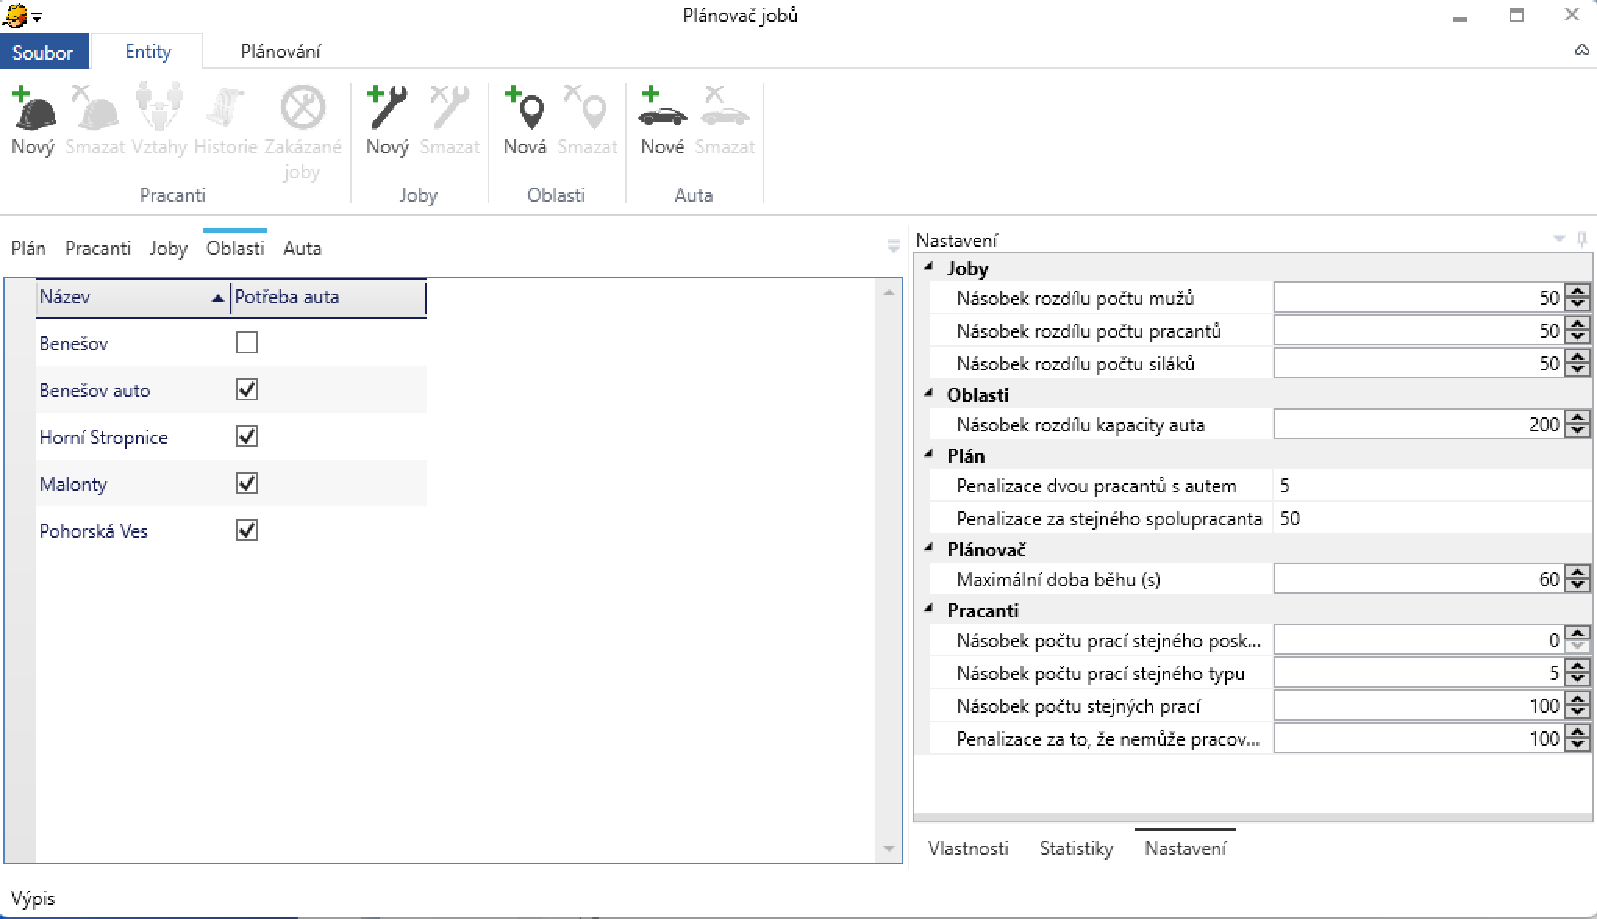
\includegraphics[width=\textwidth]{chapters/images/oldplanner}
    \caption{Současná aplikace pro evidenci a plánování}
    \label{fig:oldplanner}
\end{figure}

\section{Nevýhody současného řešení}

Na základě analýzy aplikace a konzultací s organizátory akce SummerJob byly zjištěny následující nedostatky současného řešení:

\begin{itemize}
    \item Aplikace je dostupná pouze na počítačích se systémem Windows.
    \item Aplikace neumožňuje práci více uživatelů současně.
    \item Aplikace využívá jednotný účet pro přístup k databázi pro všechny uživatele, není tedy možné rozdělit práva jednotlivým organizátorům.
    \item Spojení s databází je zajištěno přes otevřený port databáze dostupný z internetu. Toto řešení je z hlediska bezpečnosti nevhodné.
    \item Spojení s databází často vypadává. V takovém případě není možné s aplikací pracovat.
    \item Automatické plánování trvá příliš dlouho, v některých případech i minutu.
    \item Není k dispozici API pro přístup k datům.
    \item Pro každý ročník je nutné založit novou databázi a ručně překopírovat potřebná data.
    \item Webové rozhraní nabízí pouze omezenou funkcionalitu.
    \item Zdrojový kód webového rozhraní využívá proprietární nezdokumentovaný framework, což znemožňuje jeho rozšíření.
    \item Brigádníci nemají možnost zobrazit si svůj plán či upravit své osobní informace.
\end{itemize}

Vzhledem k rostoucí popularitě akce SummerJob a s tím souvisejícím rostoucím počtem účastníků se dané problémy projevují stále výrazněji.
Je tedy nutné vytvořit nové řešení, které tyto nedostatky odstraní.
